\chapter{Validation of smearing functions}\label{cha:vali}
One might assume that using a Monte Carlo simulation it would be easy to model and emulate the whole process, from collision to detection and reconstruction in the upgraded LHC. It is possible, but it requires a lot of computing power. Instead one can use one simulation and a mathematical model to calculate the estimated response in the detector. This was validated and used in this thesis to be able to create the data needed for further analysis. 

This was done by using a Monte Carlo simulation of a proton-proton collision and applying the official Truth to reco code, also known as the smearing functions, that was developed using previous studies \citep{ATLAS:LOI2, ATL-PHYS-PUB-2013-004}. to simulate how the detector and the reconstruction is affected by the increased luminosity and the pile-up that comes with this.

The code uses the experimental data from the previous studies to smear the reconstructed energy and momenta, it is from this that the name smearing functions comes.
The key feature of those studies were that the direction of the momenta does not alter direction and also that only jets and $E^{Miss}_T$ are effected by pile-up, more in \subsectionref{cha:vali:sec:results}.

\newpage
\section{Smearing functions}\label{sec:smear}
\textbf{Put in introduction? The particles that are directly detectable in \abbrATLAS are:} electron, photon, muon, tau. Aside from this jets can be detected, and from this $E_T^{Miss}$ can be calculated. This means that the all detectable entities must have their own smearing functions.

Somehow explain the entities used. 

The electron and photon have the same smearing since they are both detected in a similar way.  Perhaps add more to the introduction about each part of the detector. or simply write that here?

The smearing takes a lot into account, efficiency etc...

\section{Validation}\label{sec:vali}
To validate the smearing functions a comparison with \citep{ATL-PHYS-PUB-2013-004} was made where the standard deviation, depending on the energy of momentum value of an entity, was given, see \subsectionref{cha:vali:sec:results:subsec:expr}. To calculate this some simulated processes were needed to extract data, see \tableref{tab:backproc}. 
\begin{SCtable}[][ht]
\begin{tabular}{|l|l|}
\hline
Data & Process \\ \hline
Electron & W$\rightarrow e\nu$ \\
Muon & W$\rightarrow \mu \nu$ \\
Tau & W$\rightarrow \tau \nu$ \\
$\gamma$ & $\gamma$ + Jet sample \\
Jets & Jet sample \\
$E_T^{Miss}$ & Z$\rightarrow \nu \nu$ + Jet sample \\ \hline
\end{tabular}
\caption{Different processes from where data has been taken. Each sample is a simulation of a physical process, the simulation names can be found in \appendixref{cha:datasets}}
\label{tab:backproc}
\end{SCtable}

By plotting the data for each data point before and after the smearing function, denoted truth and reco, for that data point had been used, one could verify the functions. It was done looking at the reco data for a given truth energy or momentum value. The reco data will be spread out, since there should be effects \textbf{explain more about effeciency, why spread?!}. 

Trying to fit a Gaussian curve to this data will then result in the mean value, and the standard deviation. The mean value is not of interest for the purposes of the thesis, though it is this standard deviation which is compared. 


\section{Results}\label{cha:vali:sec:results}
As discussed in validation, the method was to plot the data against its smeared counterpart and through this determine the standard deviation to see if it conforms to the expected values.

Since there are very slight differences depending on pile-up these are not shown except for met and jets. Also only one energy value is shown for all but electrons for simplicity. Though all were checked.
\subsection{Electron and photon}
Since these interact very  similarly in the detector, their smearing functions are identical.
 \begin{figure}[H] %!ht
    \subfloat[eleta1. \label{fig:elph:1}]{%
     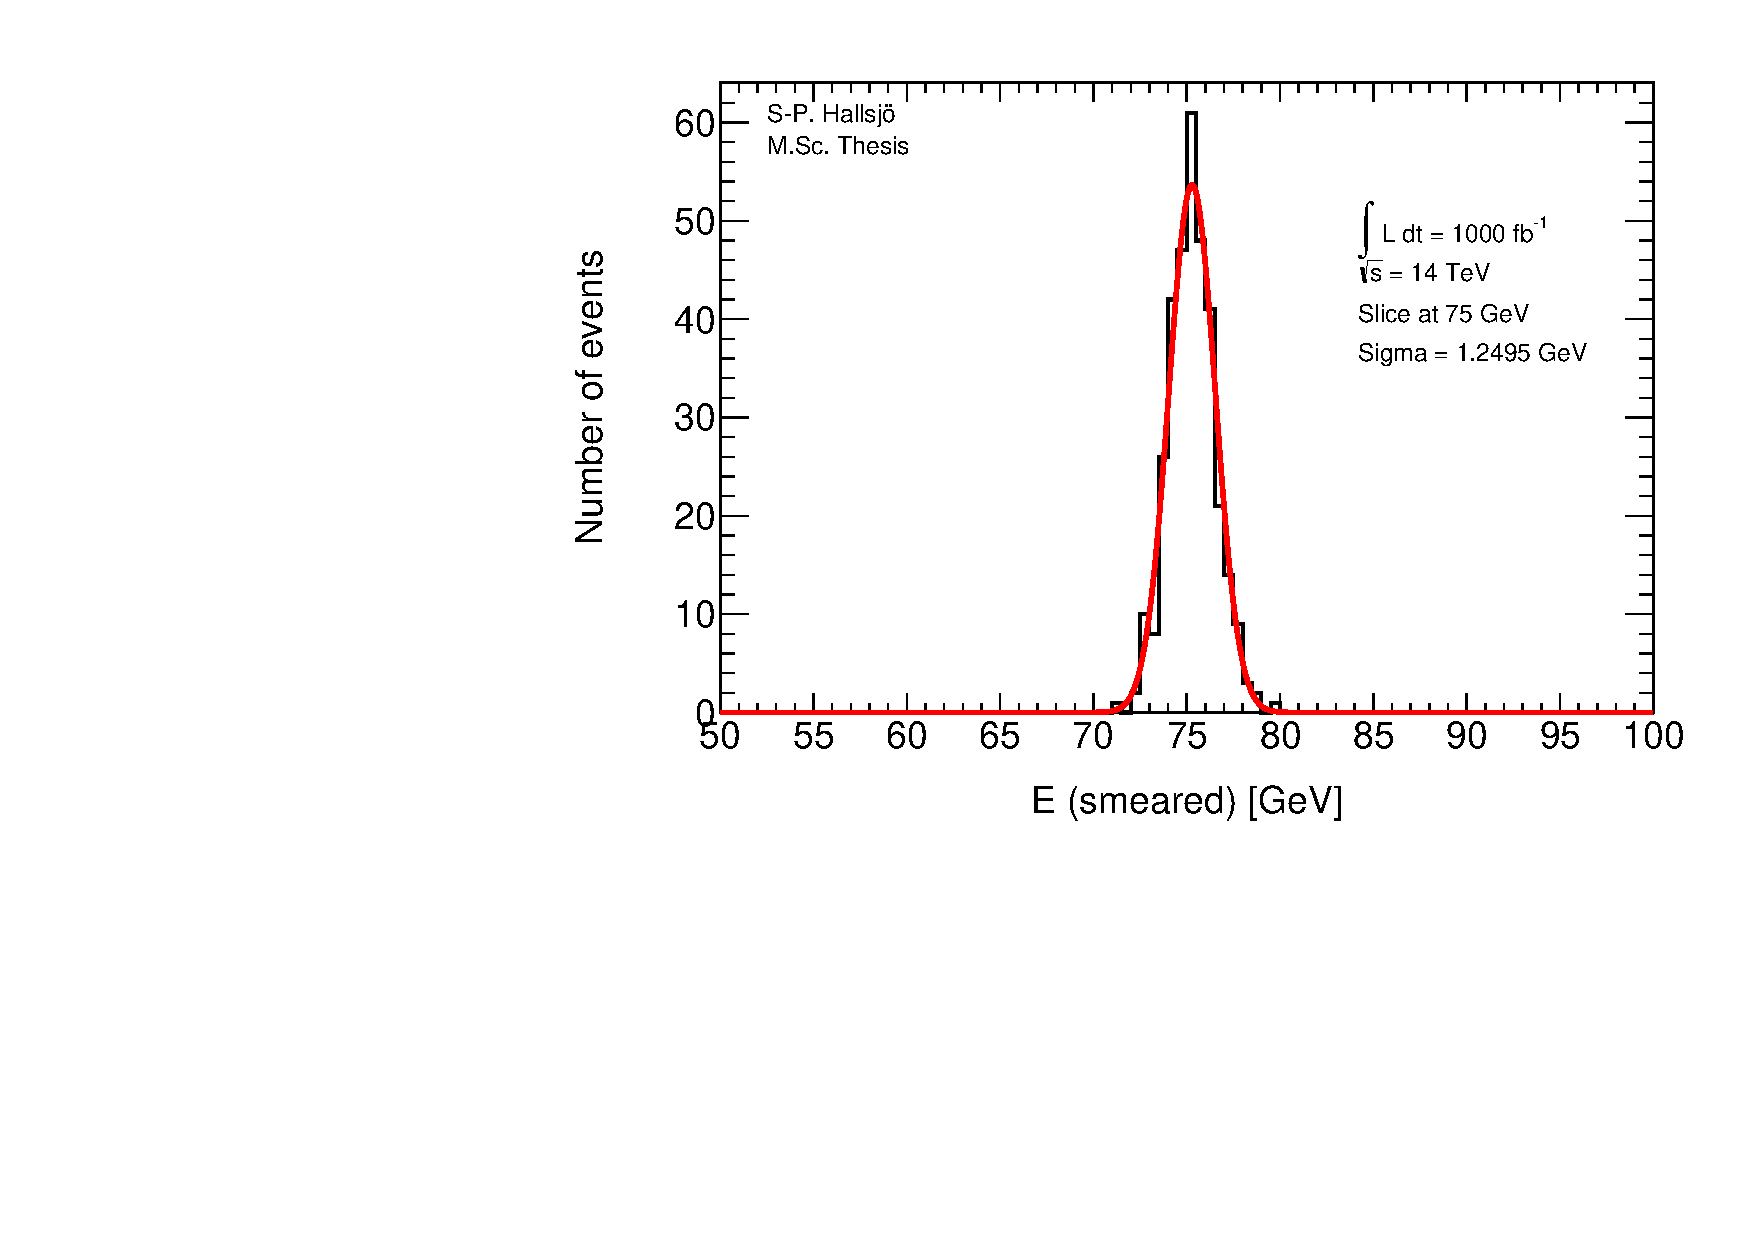
\includegraphics[width=0.5\textwidth]{eleta1.pdf}
    }
    \hfill
\subfloat[eleta2.\label{fig:elph:2}]{%
      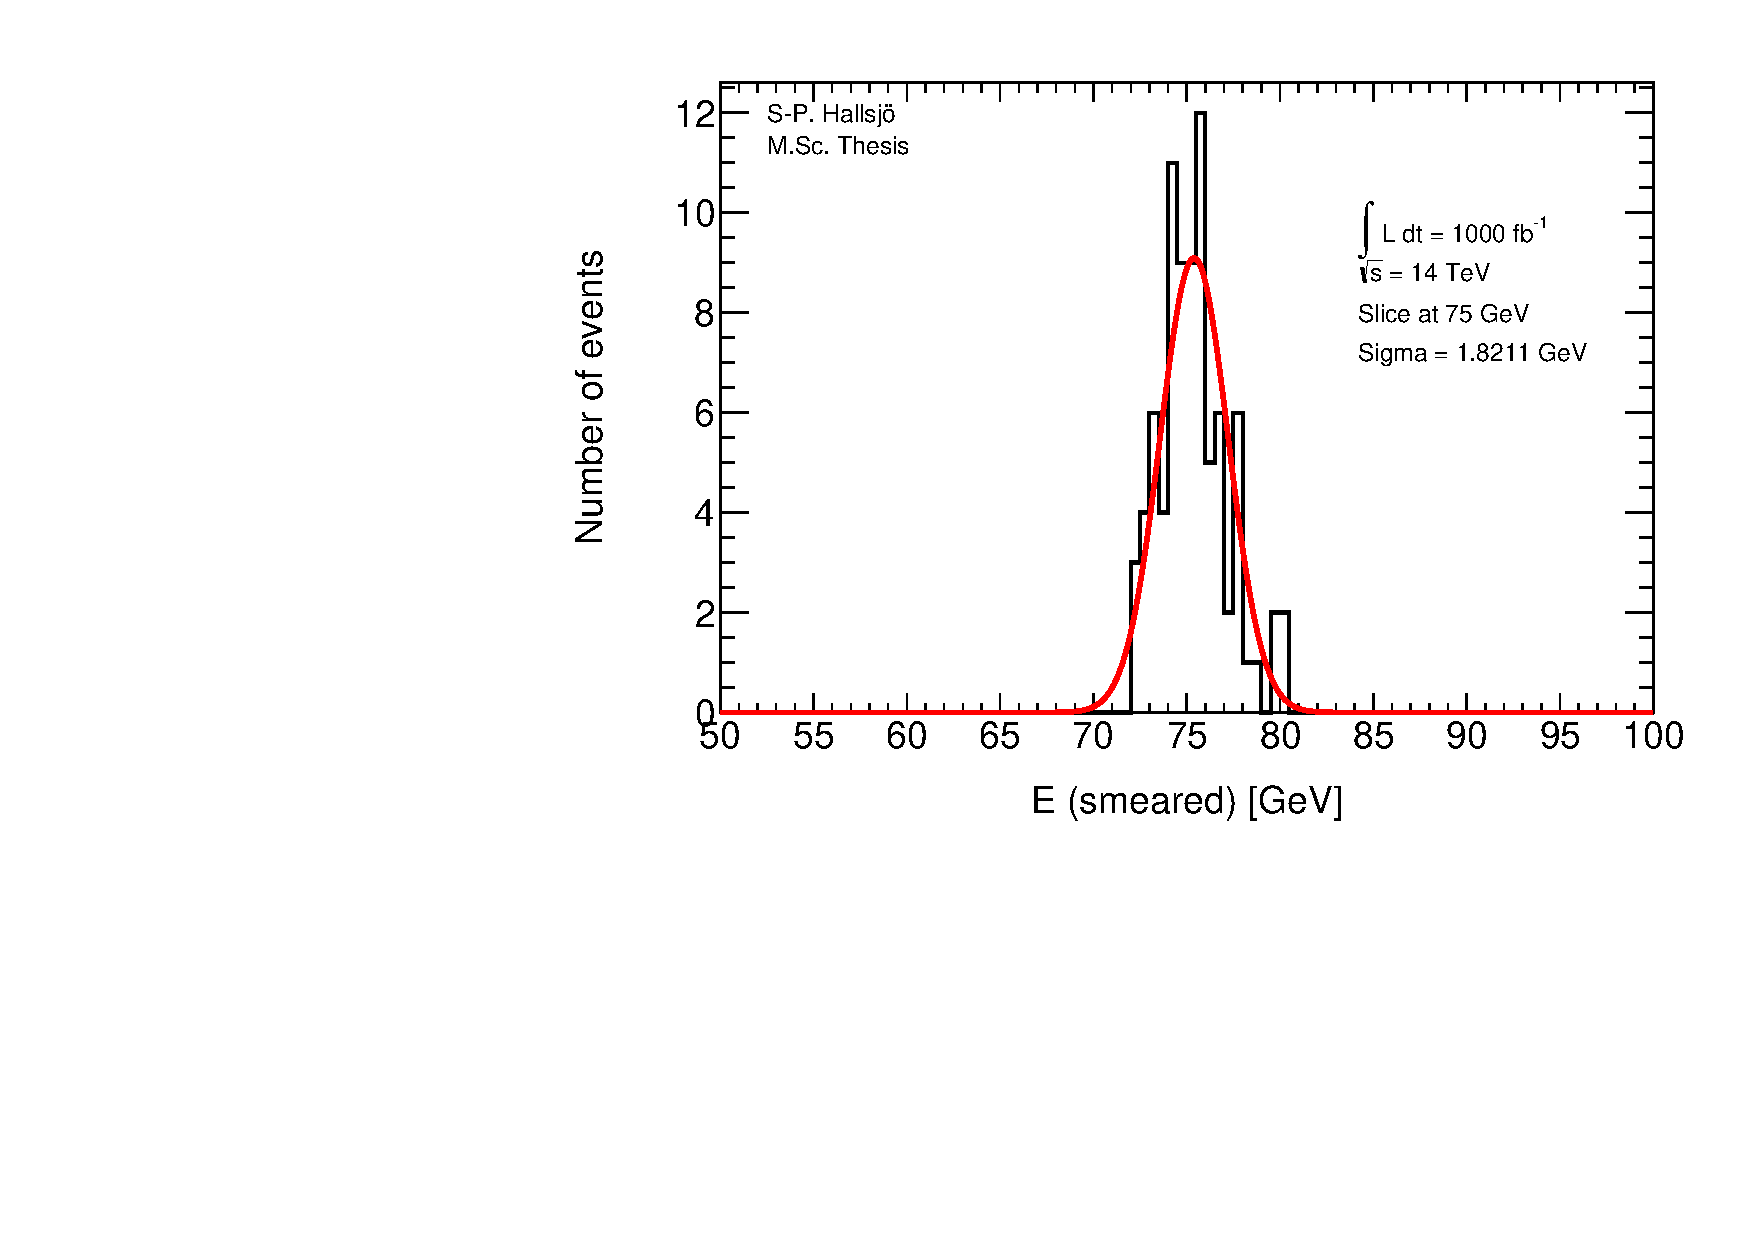
\includegraphics[width=0.5\textwidth]{eleta2.pdf}
    }
    \hfill
        \subfloat[pheta1. \label{fig:elph:3}]{%
     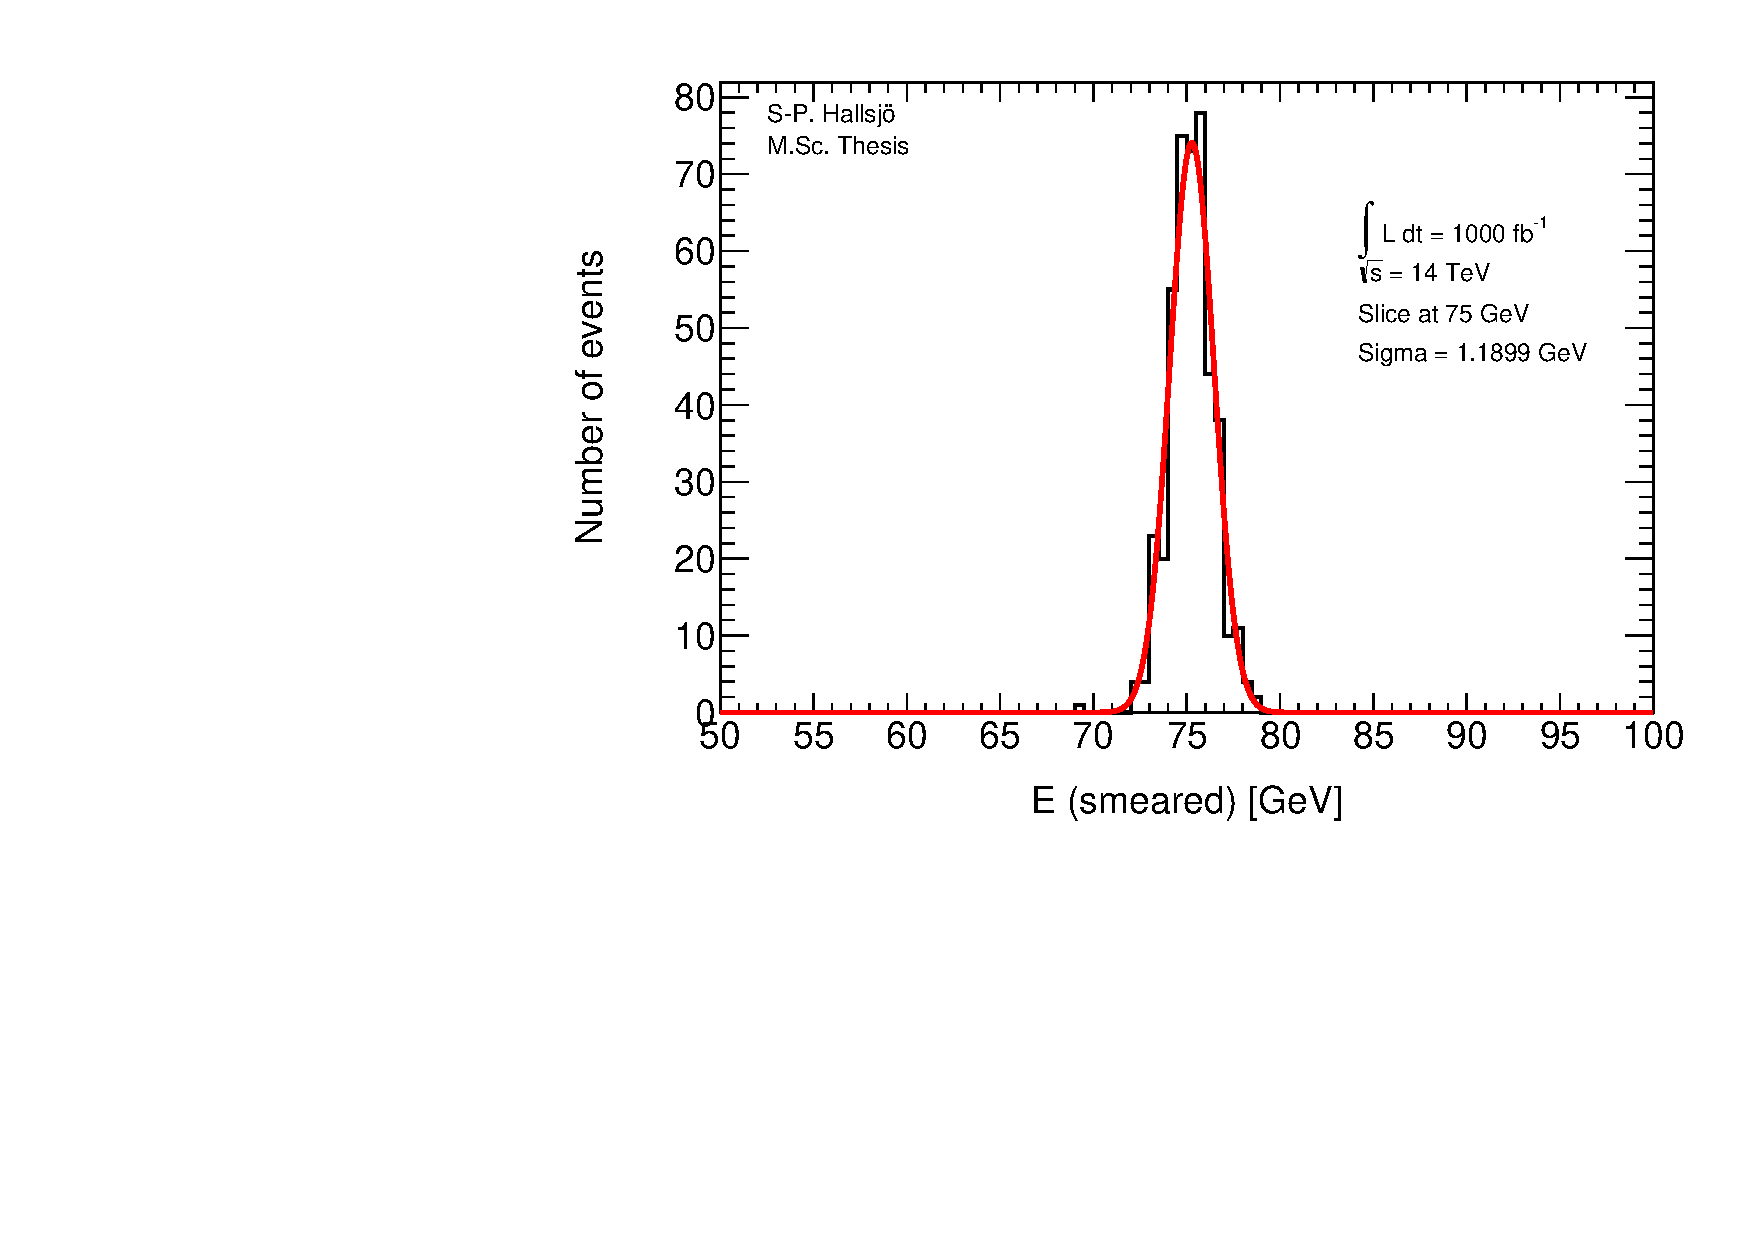
\includegraphics[width=0.5\textwidth]{pheta1.pdf}
    }
    \hfill
\subfloat[pheta2.\label{fig:elph:4}]{%
      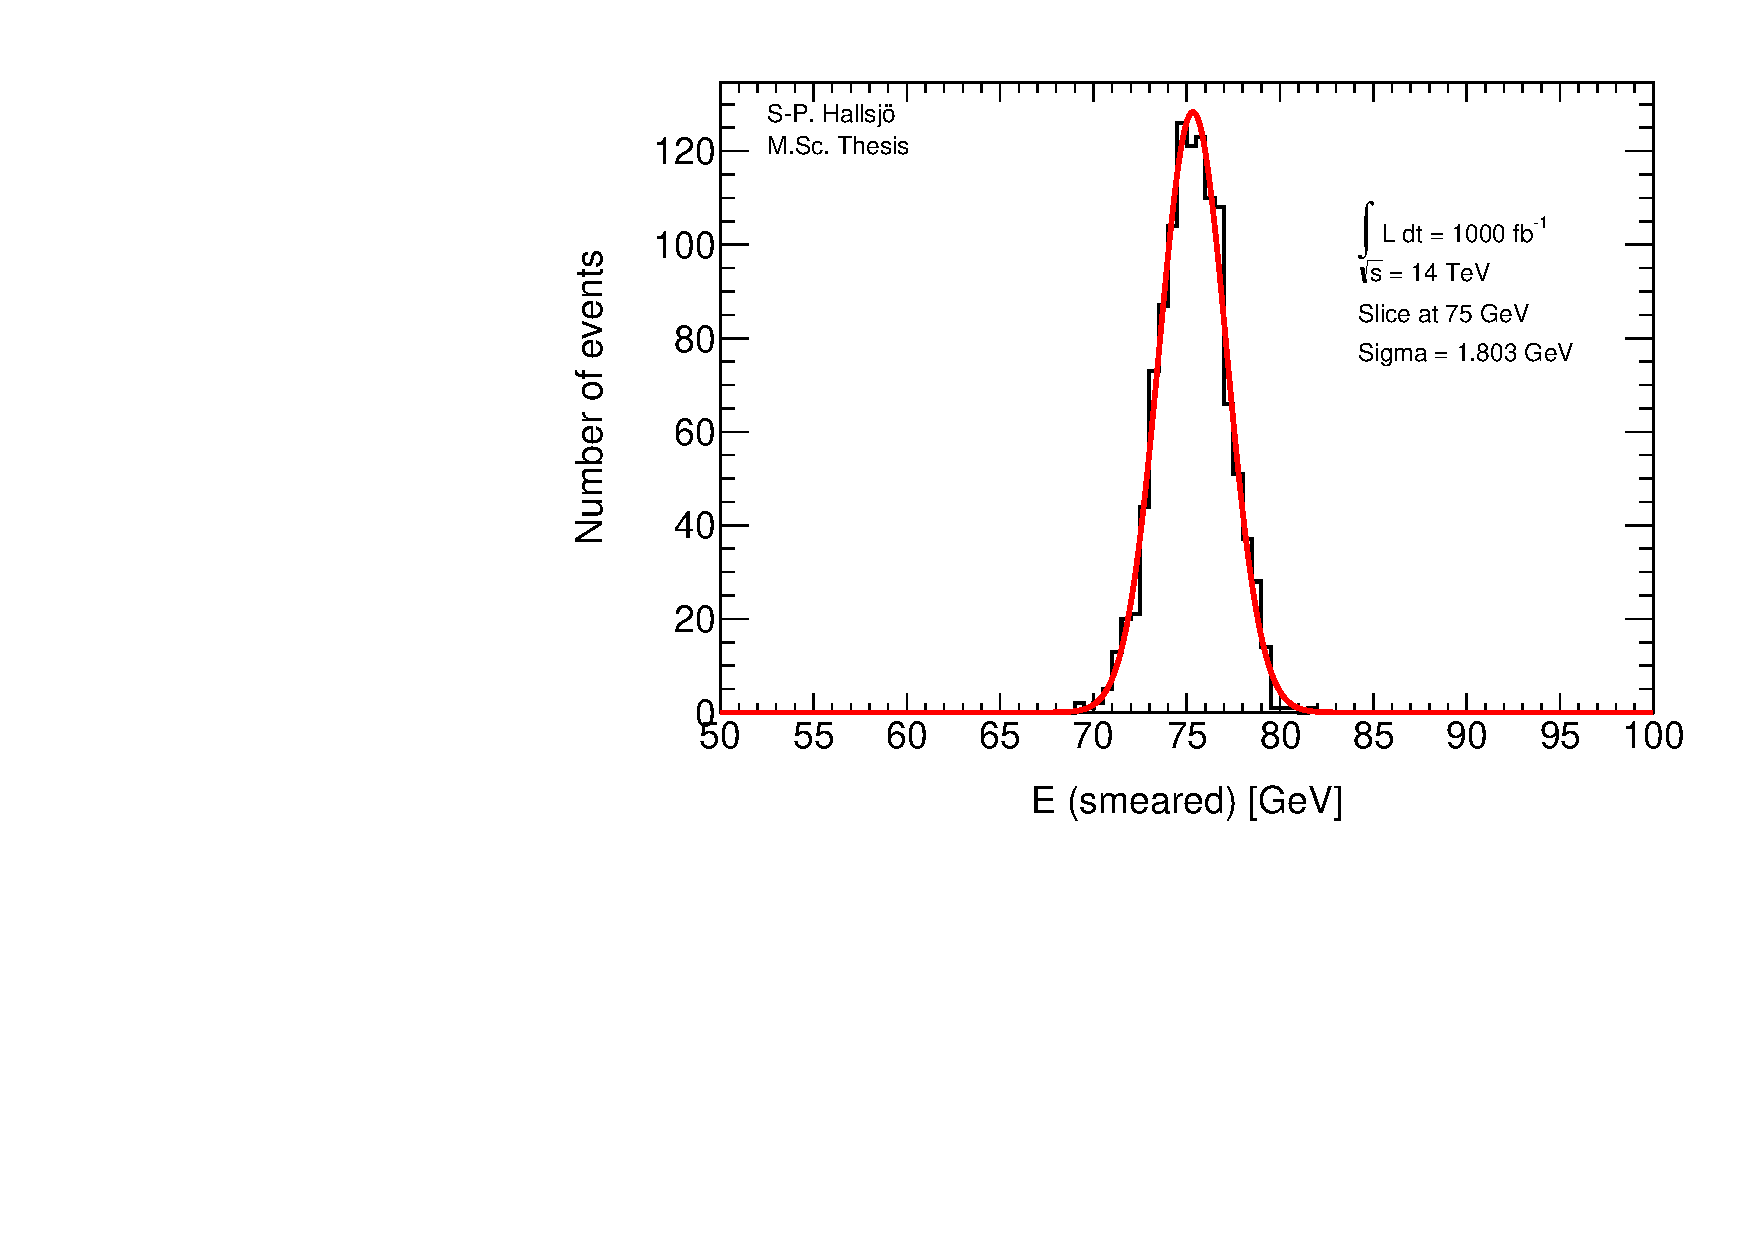
\includegraphics[width=0.5\textwidth]{pheta2.pdf}
    }
    \caption{el and ph eta}
    \label{fig:elph}
\end{figure}
\subsection{Muon}
 \begin{figure}[H] %!ht
    \subfloat[Muoneta1. \label{fig:muon:1}]{%
     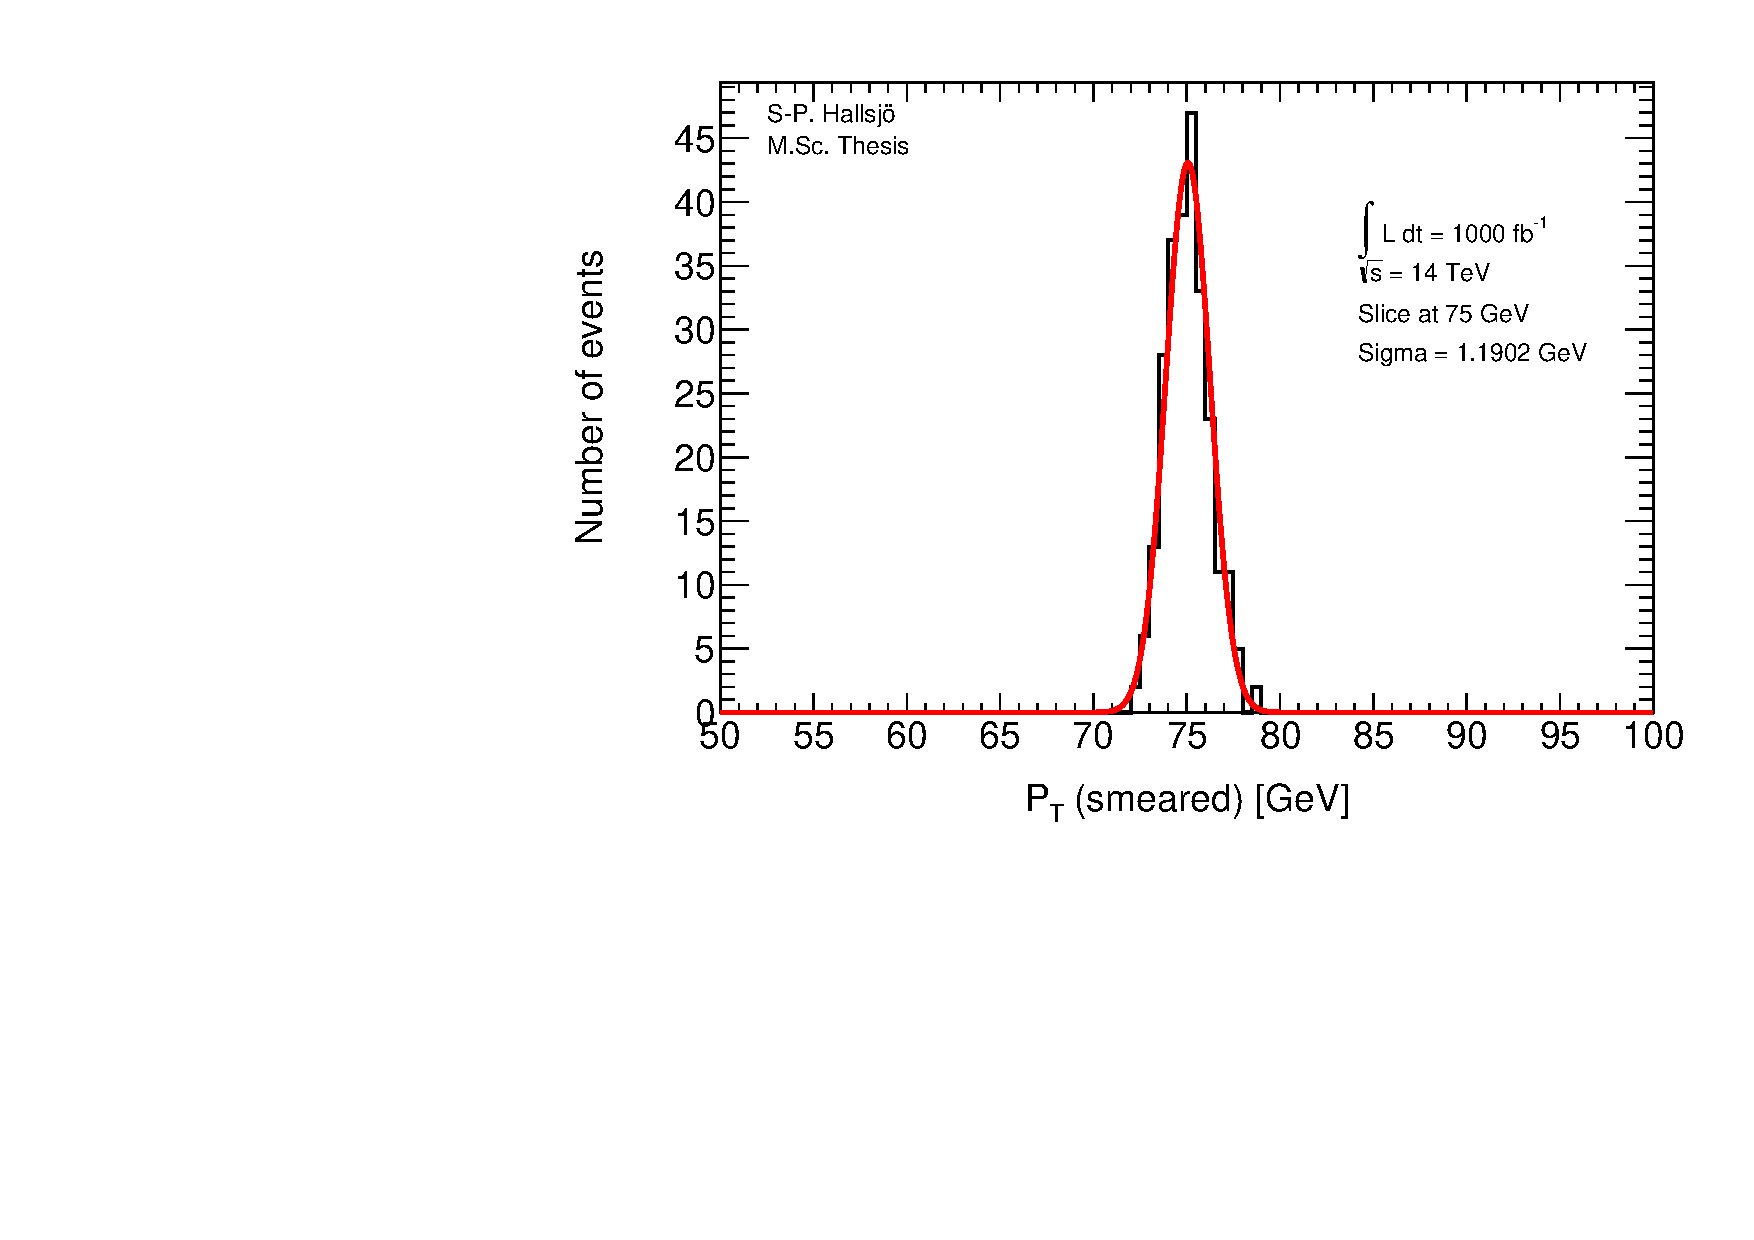
\includegraphics[width=0.5\textwidth]{mueta1.pdf}
    }
    \hfill
    \subfloat[Muoneta2.\label{fig:muon:2}]{%
      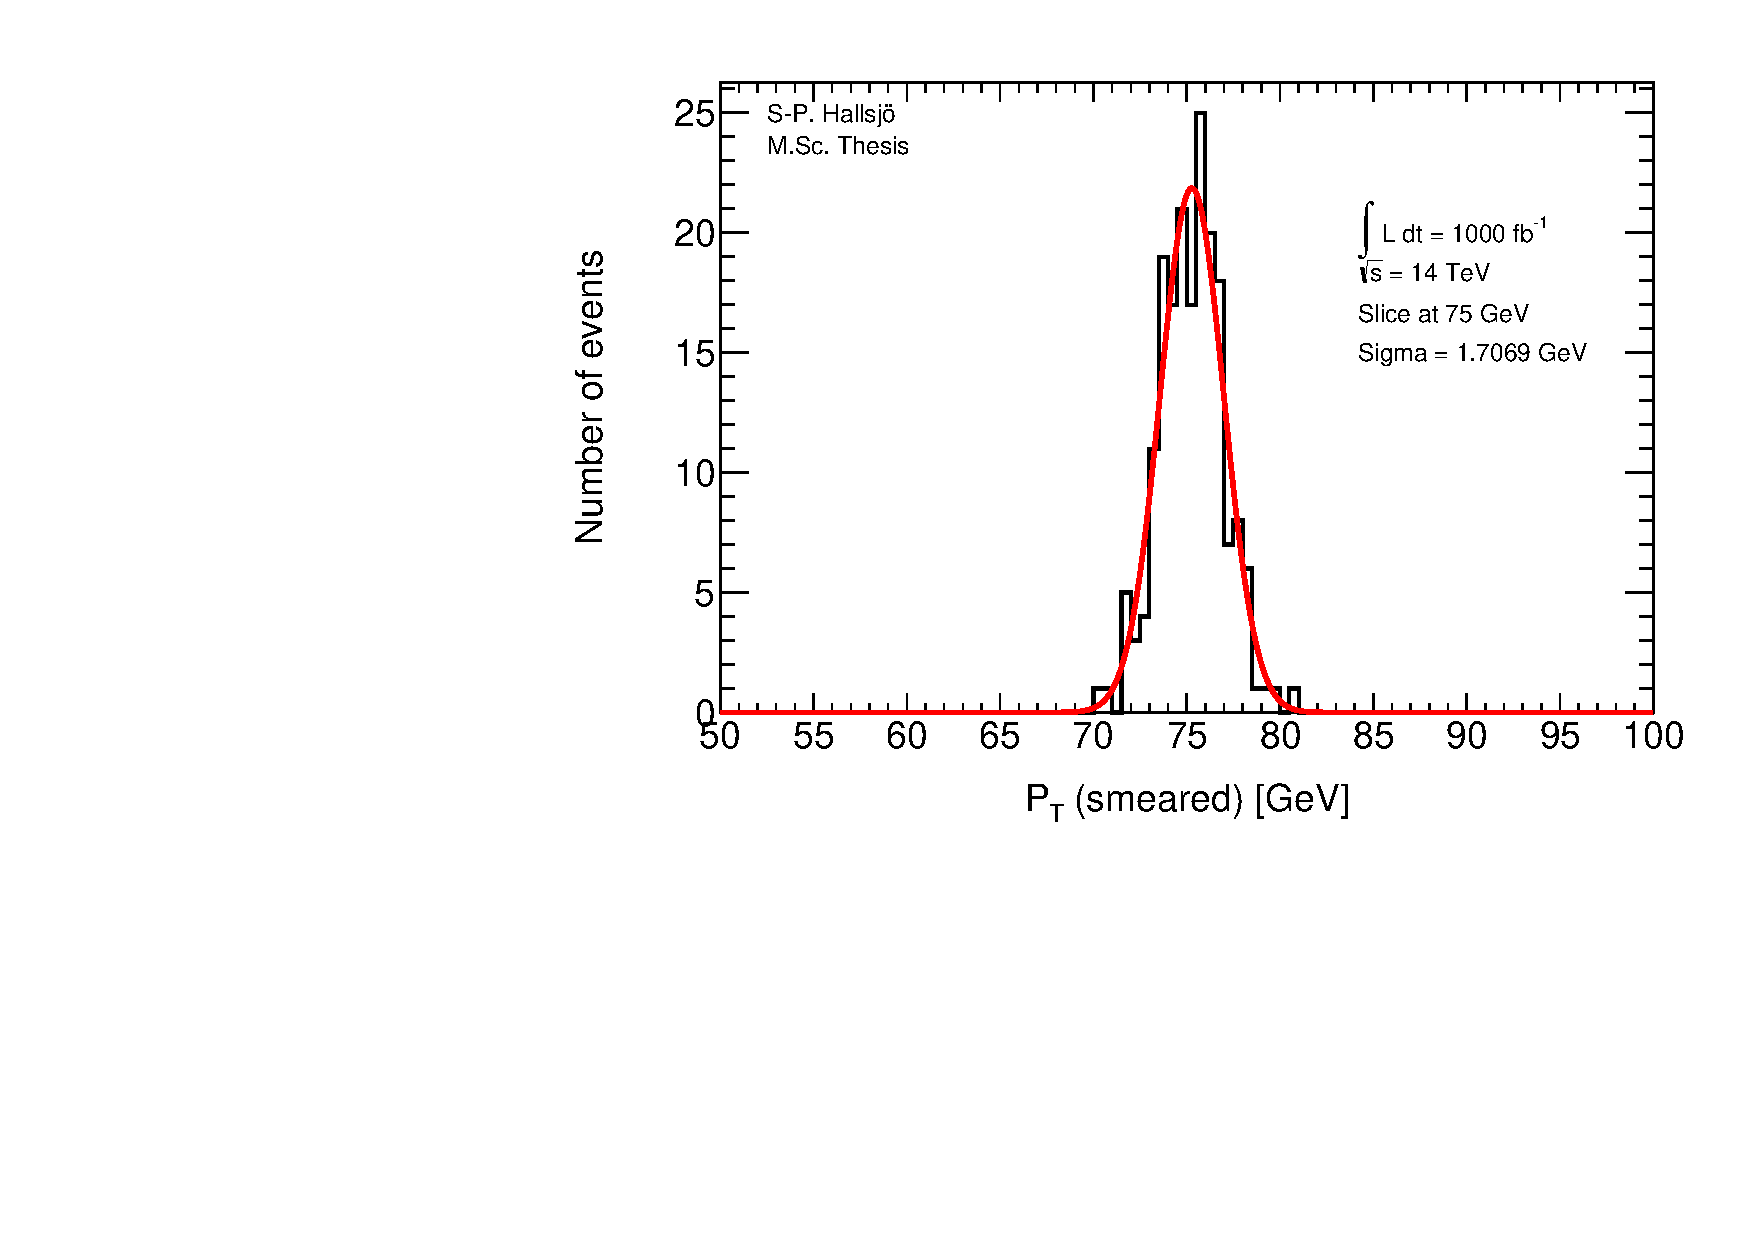
\includegraphics[width=0.5\textwidth]{mueta2.pdf}
    }
    \caption{Muon}
    \label{fig:muon}
  \end{figure}

\subsection{Tau}
 \begin{figure}[H] %!ht
    \subfloat[Tau \label{fig:tau:1}]{%
     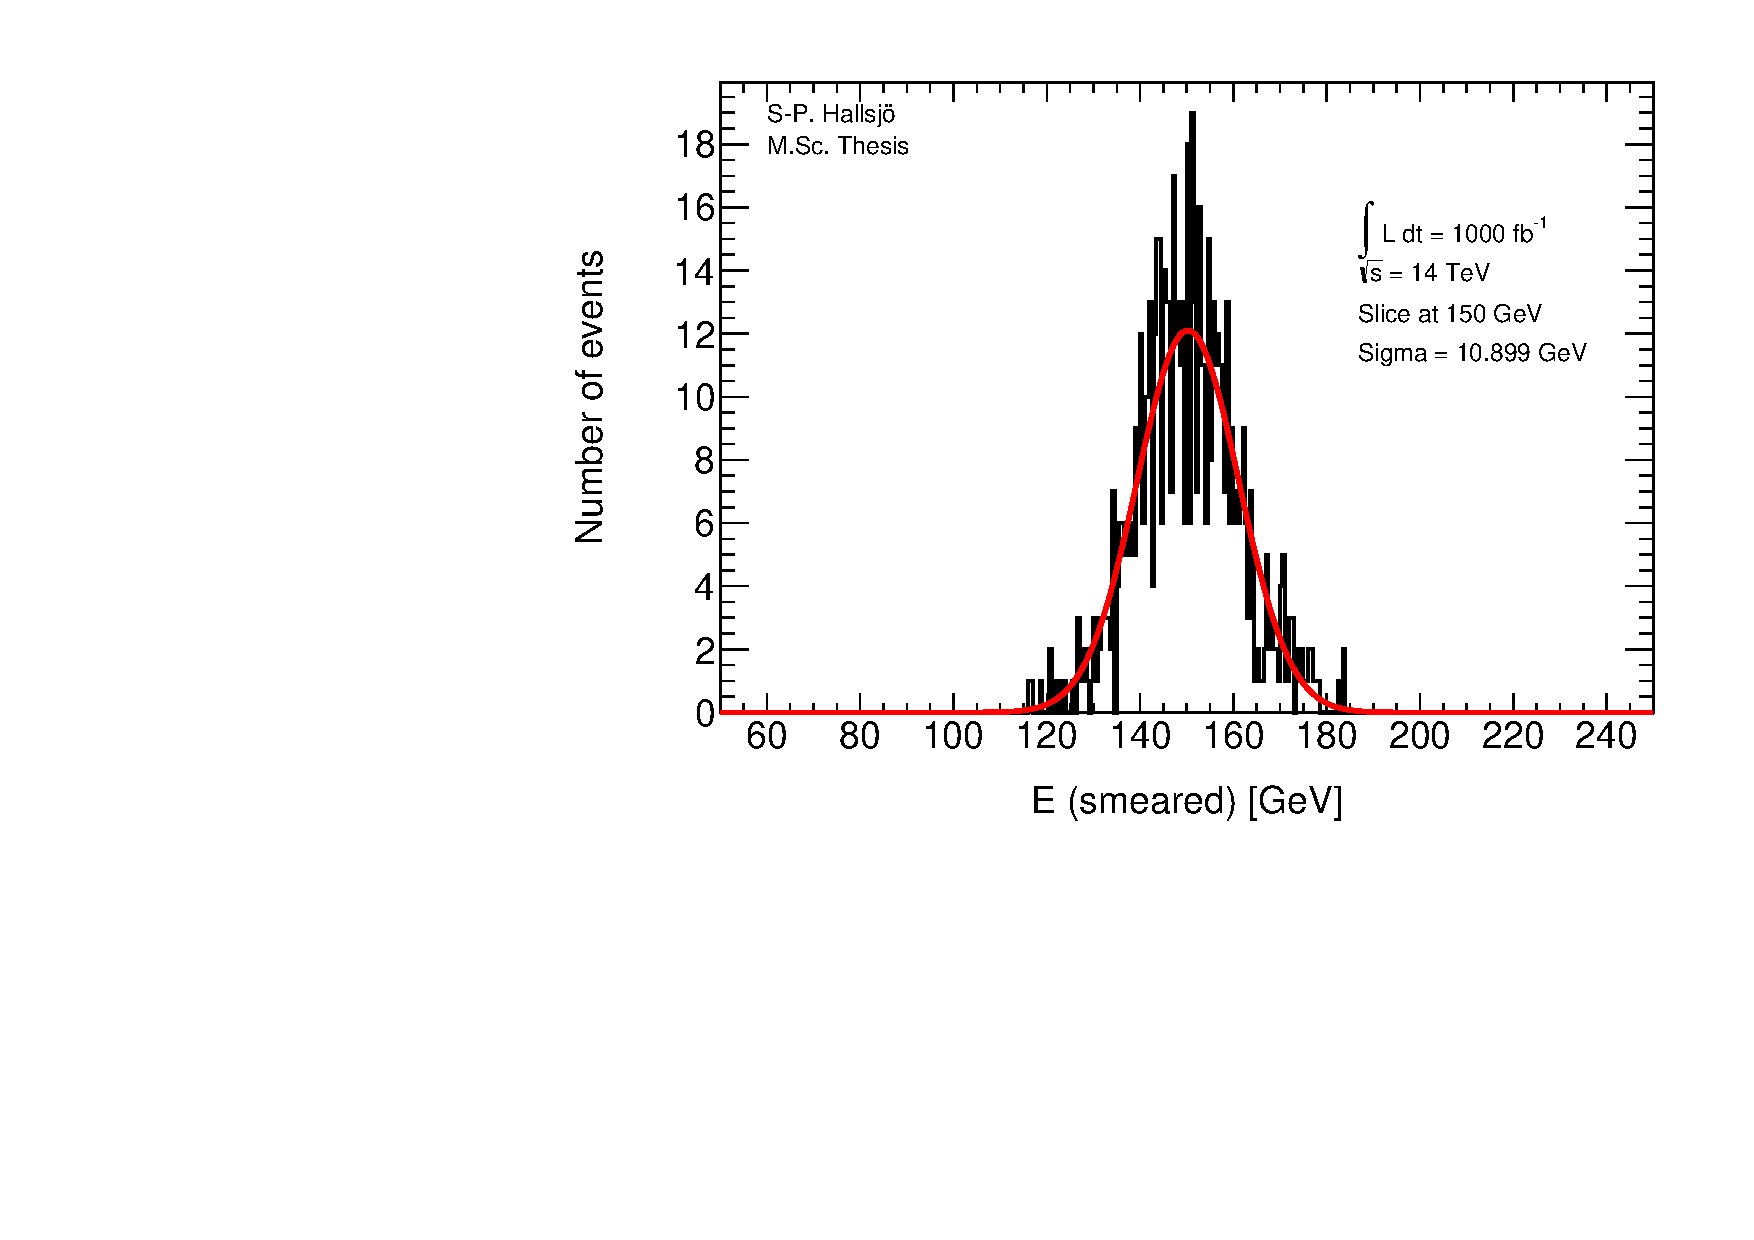
\includegraphics[width=0.5\textwidth]{tau.pdf}
    }
    \hfill
    \subfloat[Tau energy vs smeared. \label{fig:tau:2}]{%
      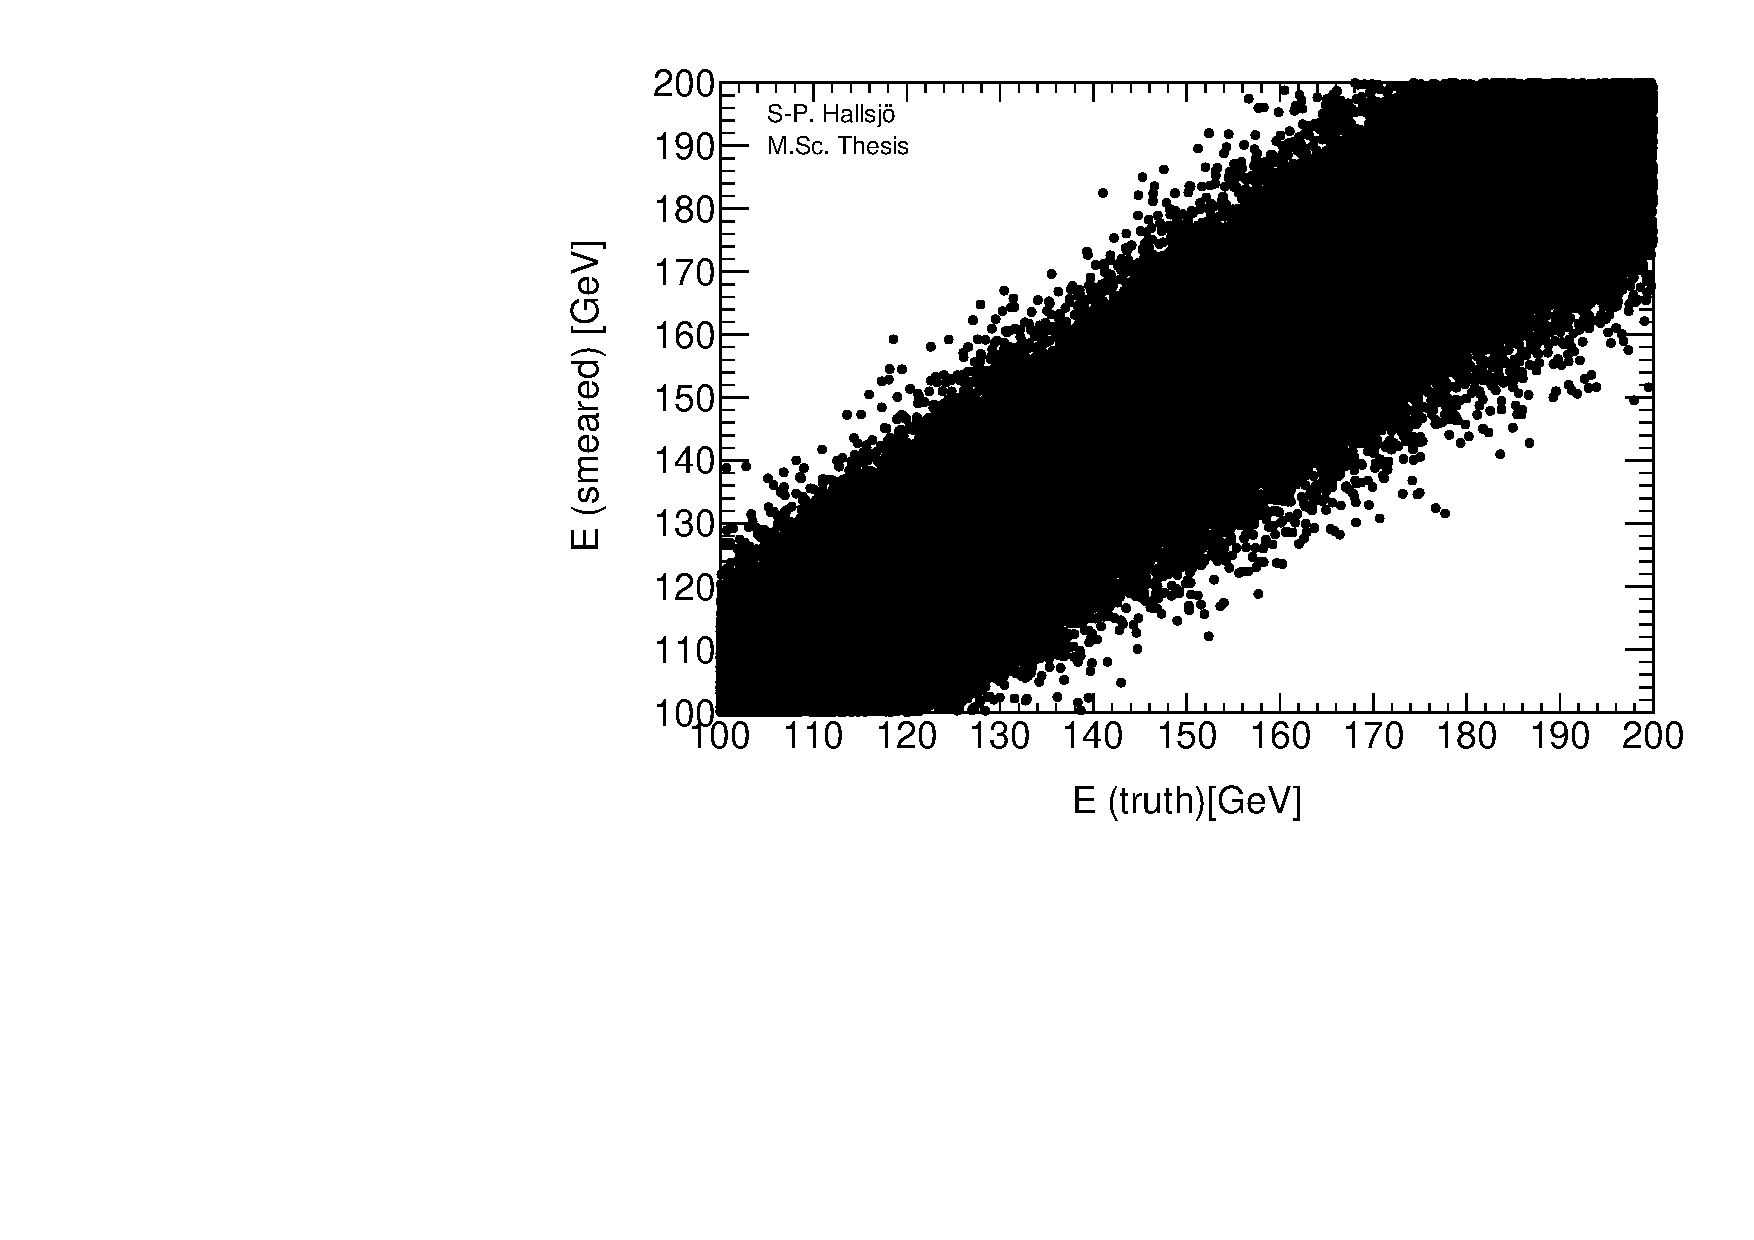
\includegraphics[width=0.5\textwidth]{tau2.pdf}
    }
    \caption{Tau}
    \label{fig:tau}
  \end{figure}
\subsection{Jets}
 \begin{figure}[H] %!ht
    \subfloat[jeteta1. \label{fig:jet:1}]{%
     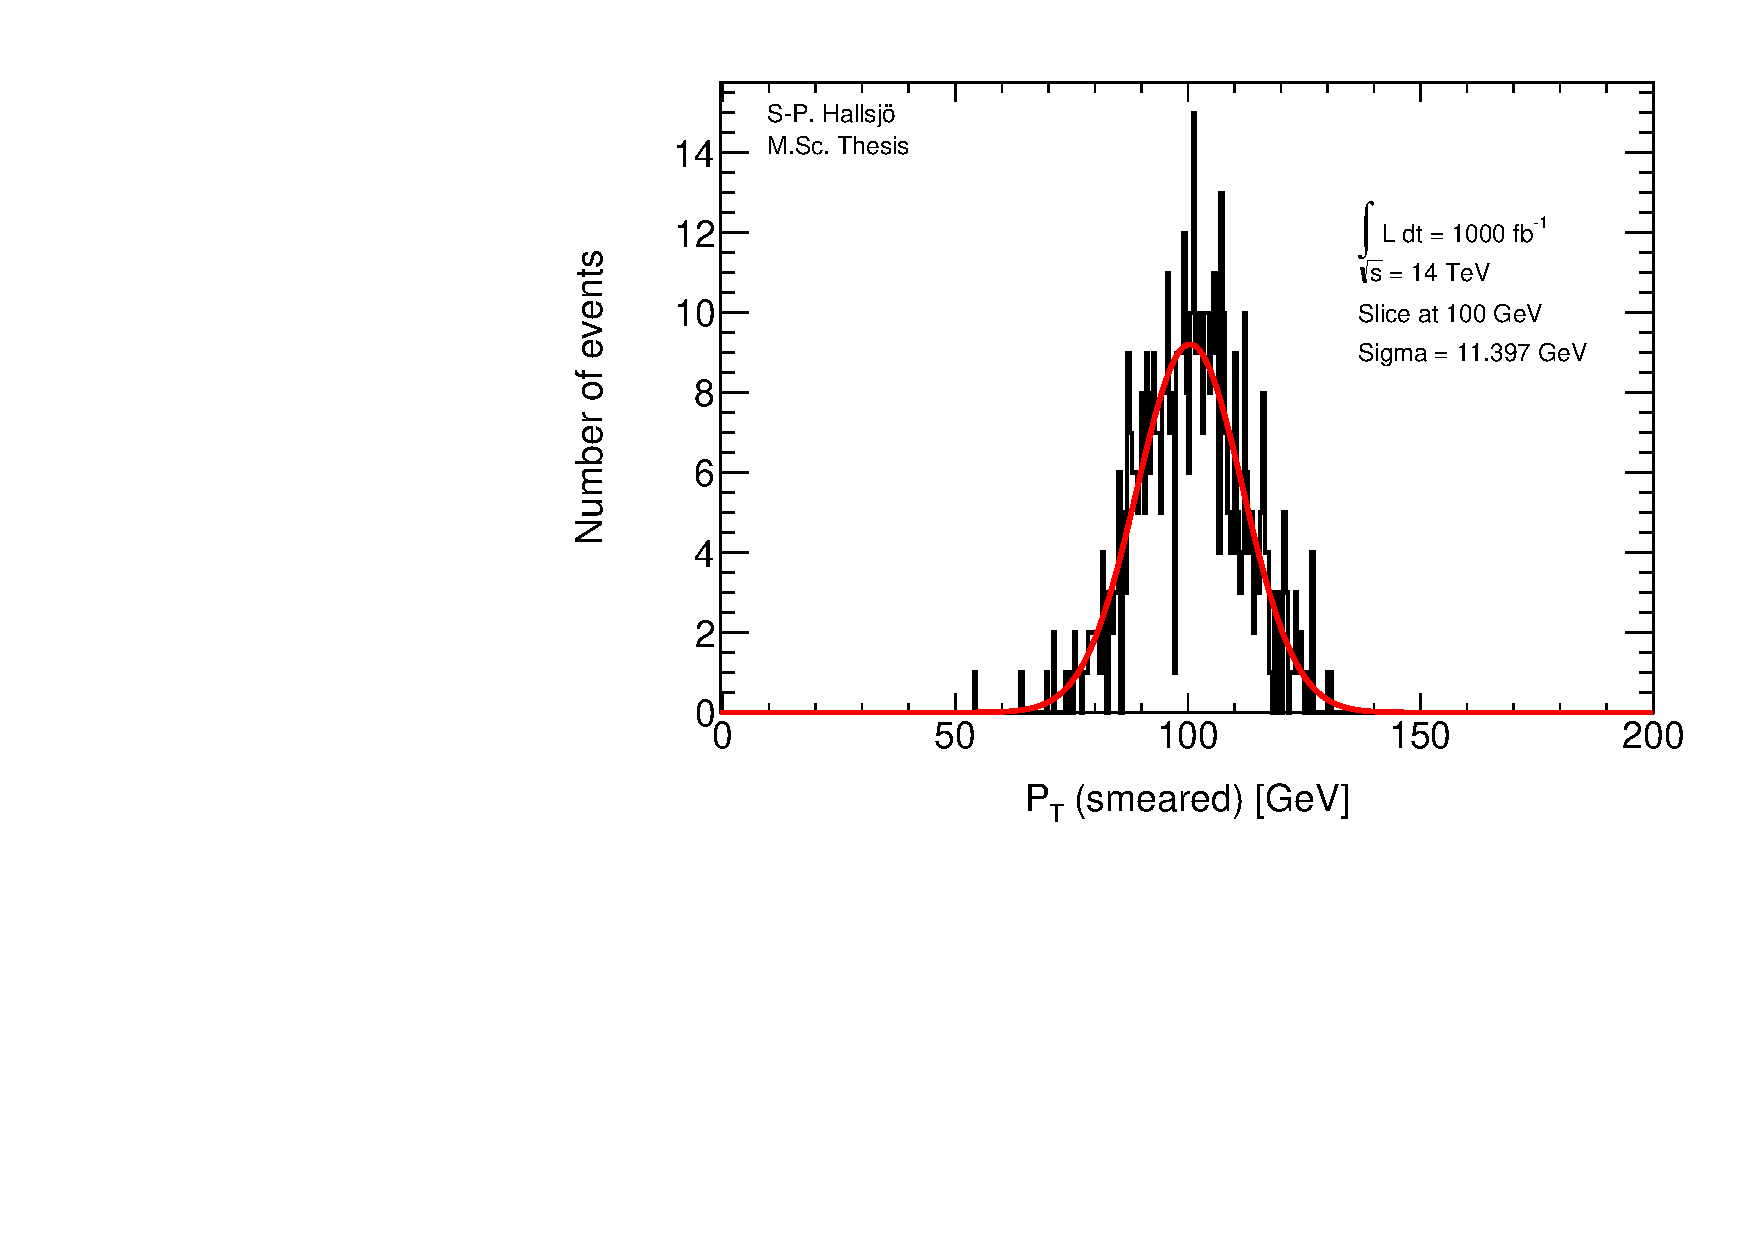
\includegraphics[width=0.5\textwidth]{jeteta1.pdf}
    }
    \hfill
\subfloat[jeteta2.\label{fig:jet:2}]{%
      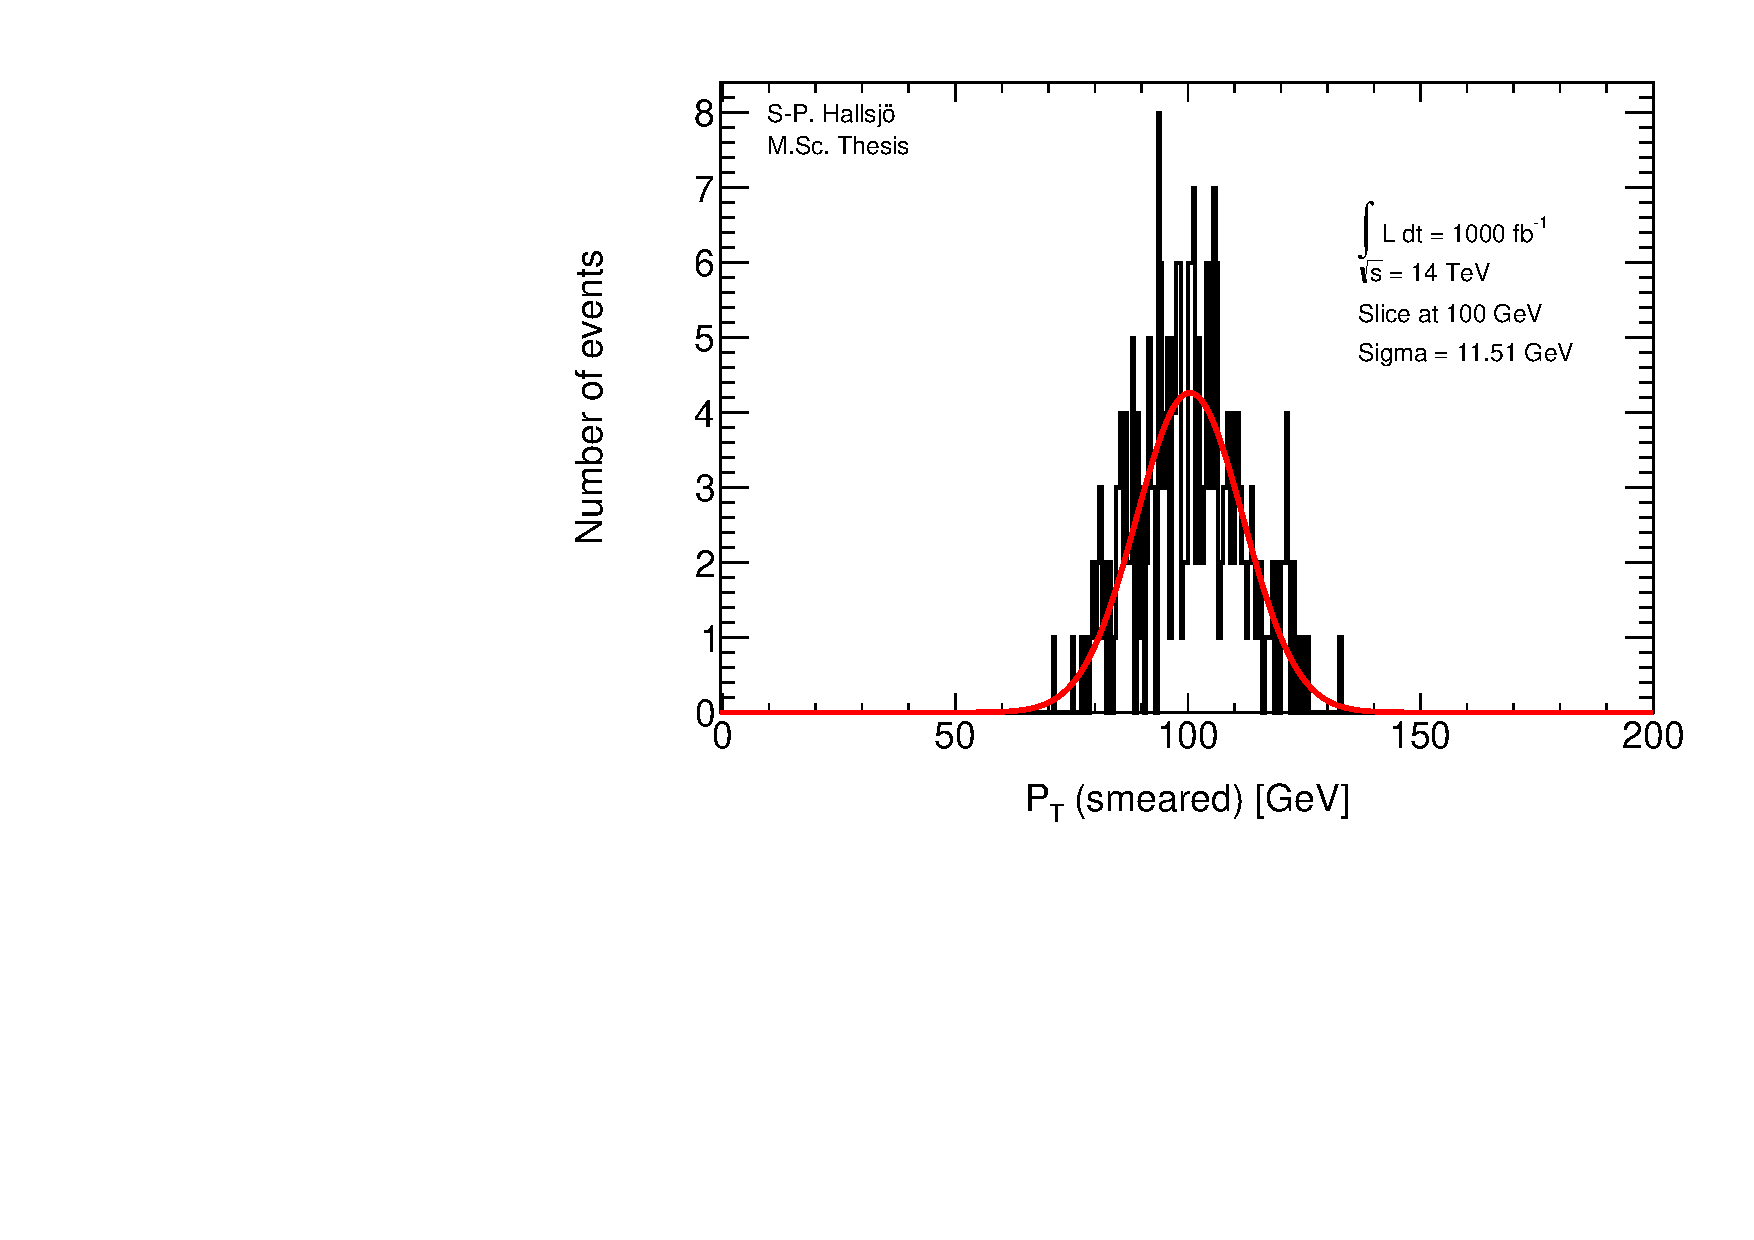
\includegraphics[width=0.5\textwidth]{jeteta2.pdf}
    }
    \hfill
        \subfloat[jeteta3. \label{fig:jet:3}]{%
     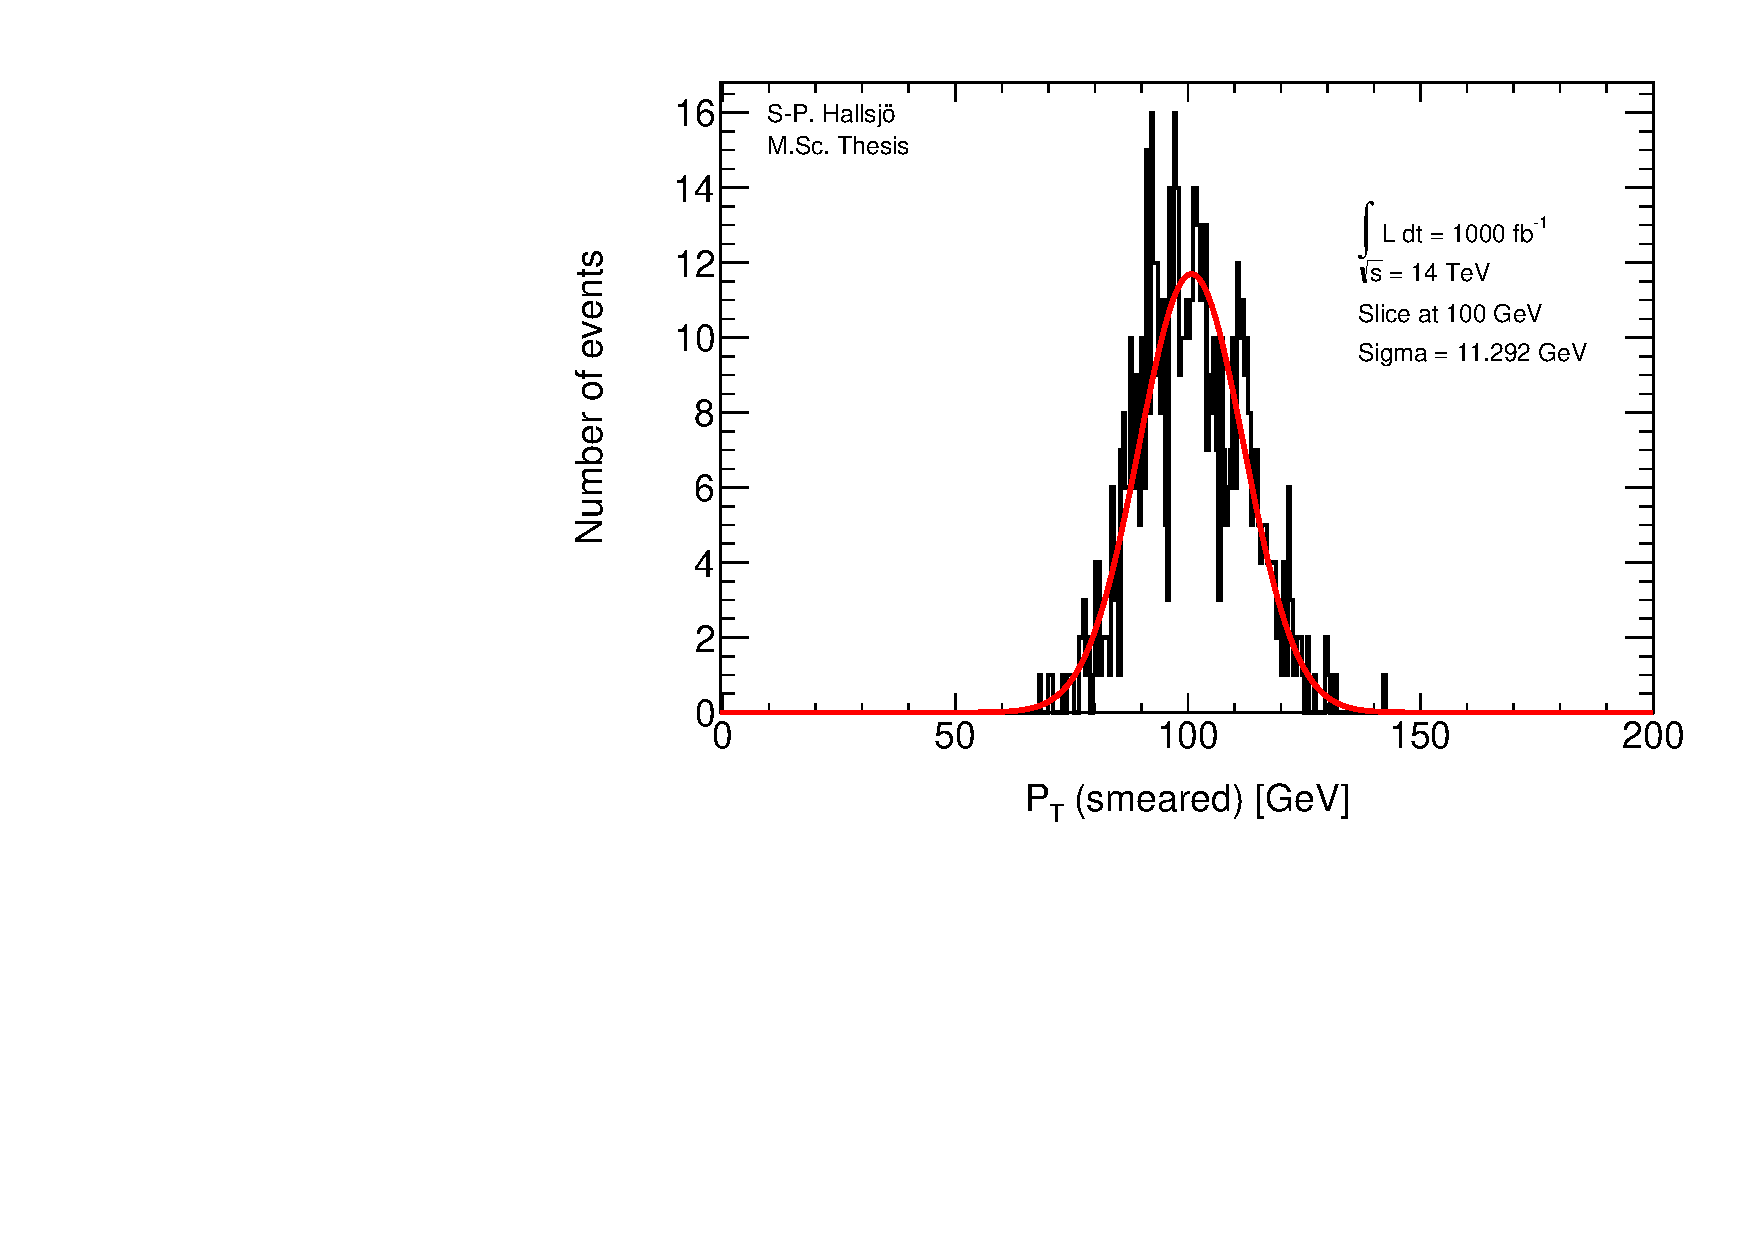
\includegraphics[width=0.5\textwidth]{jeteta3.pdf}
    }
    \hfill
\subfloat[jeteta4.\label{fig:jet:4}]{%
      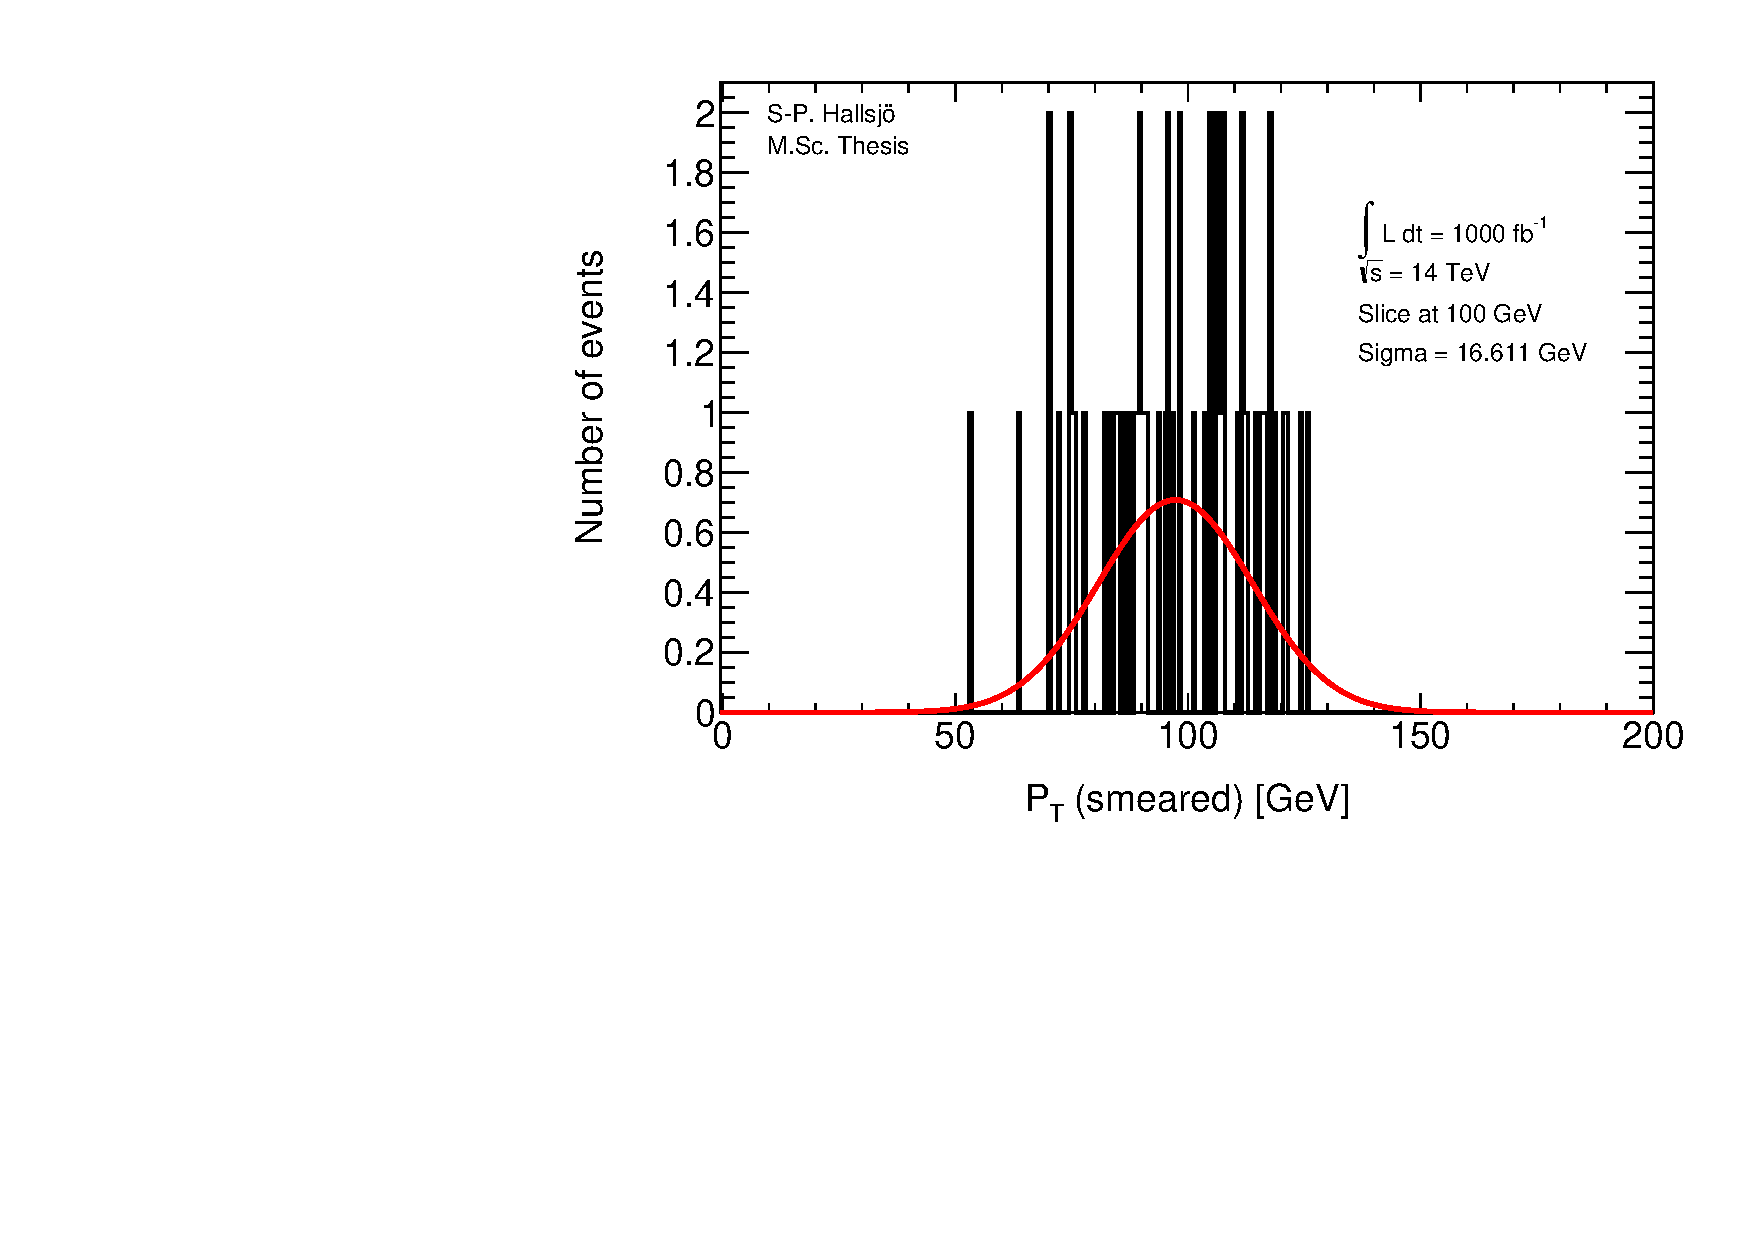
\includegraphics[width=0.5\textwidth]{jeteta4.pdf}
    }
    \caption{Jet}
    \label{fig:jet}
\end{figure}

\subsection{Missing Energy}
These figures are given as smeared value from origin, thus at 0 it represents that the energy is unsmeared, compared to the others where the slice value represents the unsmeared. 
 \begin{figure}[H] %!ht
    \subfloat[METx. \label{fig:MET:x}]{%
     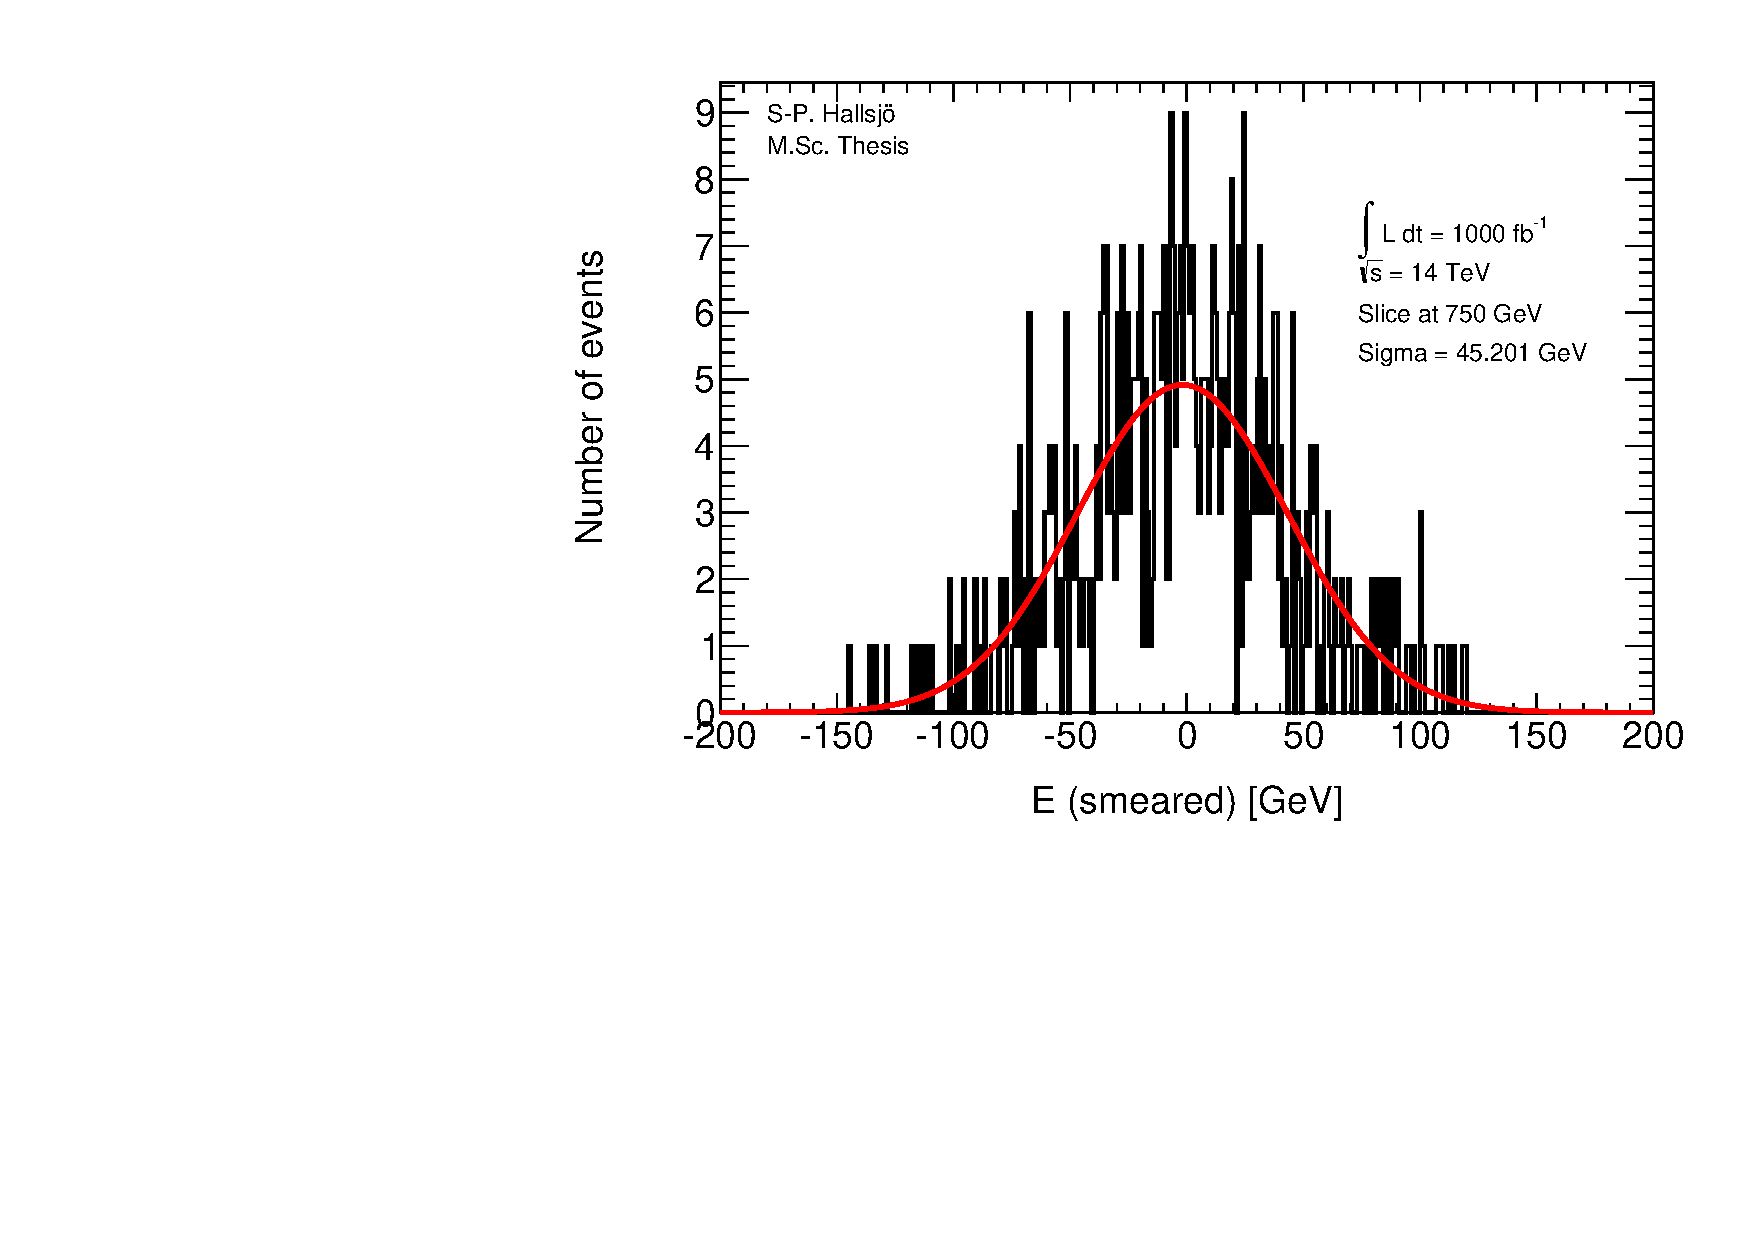
\includegraphics[width=0.5\textwidth]{METx.pdf}
    }
    \hfill
    \subfloat[METy.\label{fig:MET:y}]{%
      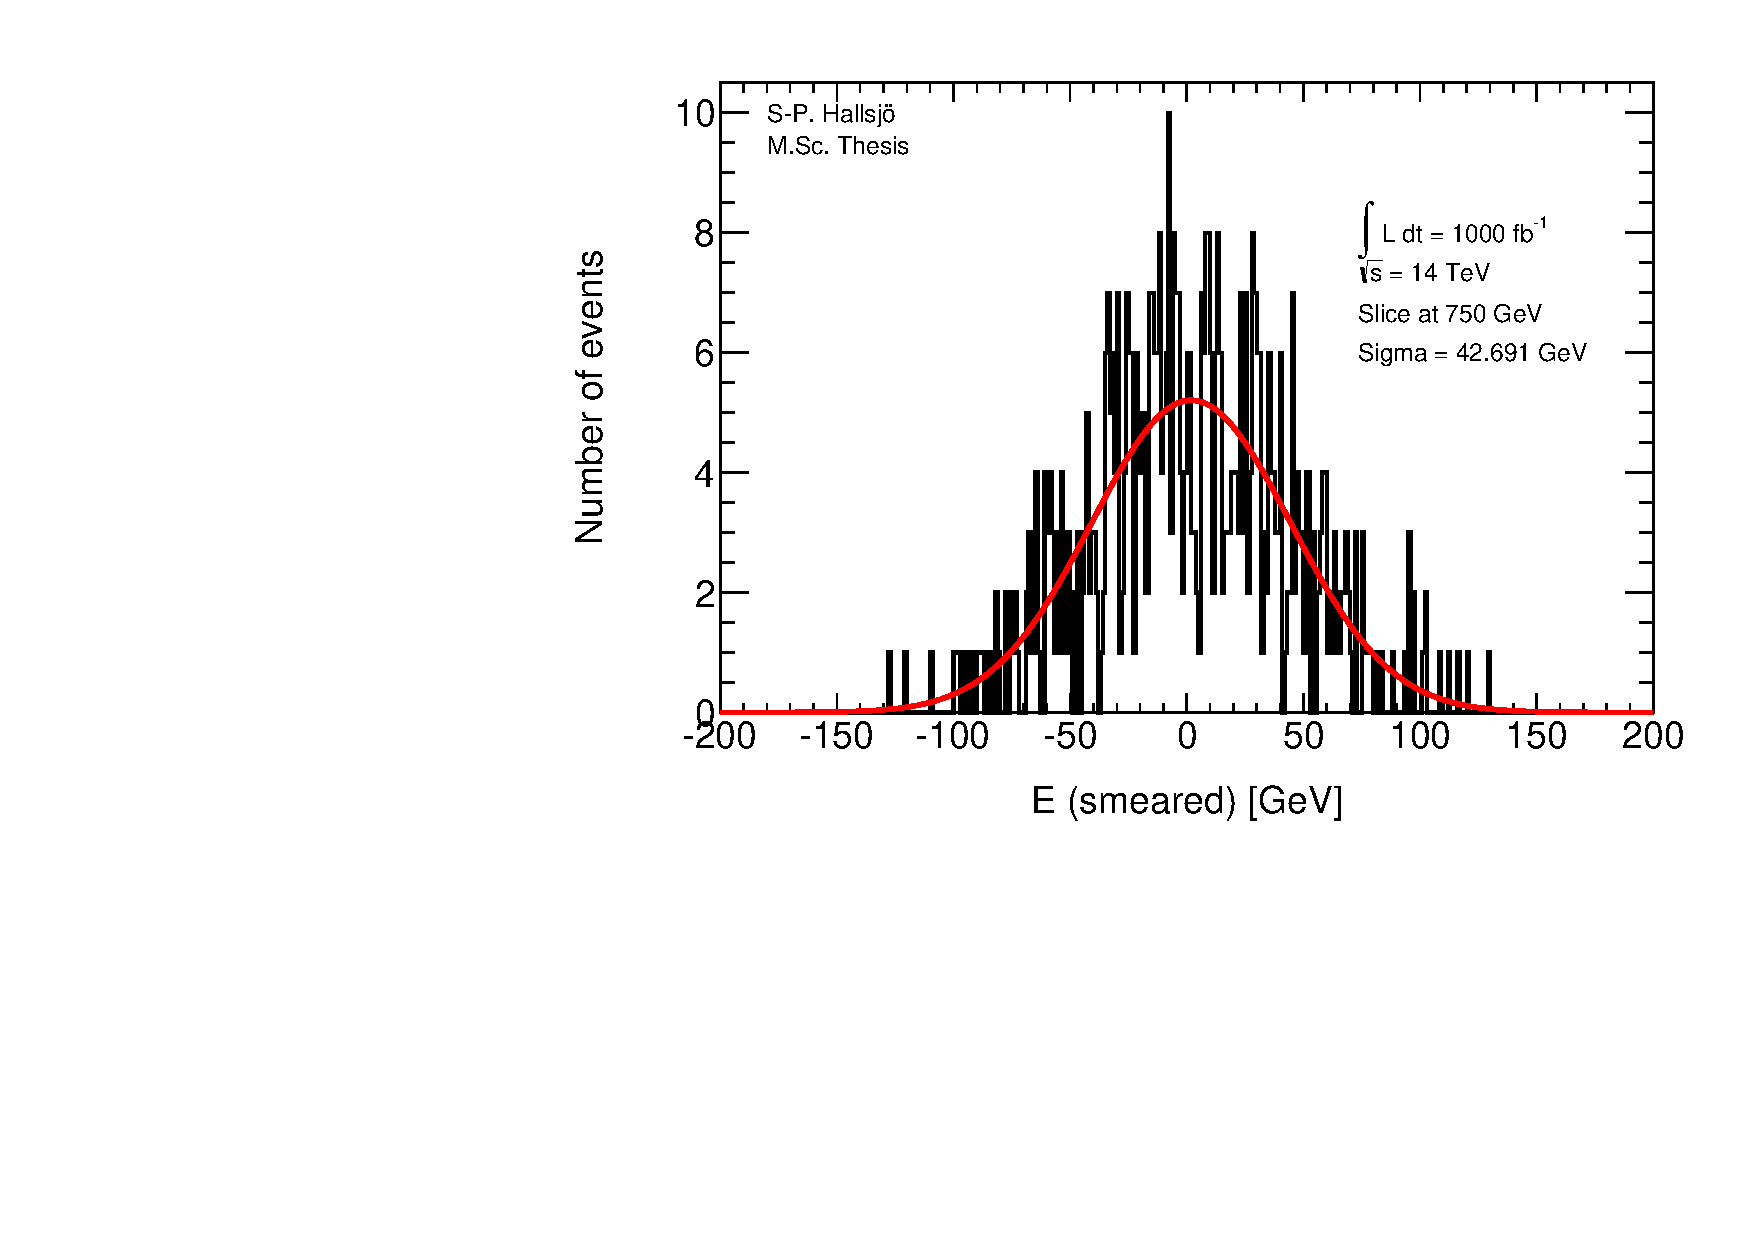
\includegraphics[width=0.5\textwidth]{METy.pdf}
    }
    \caption{MET}
    \label{fig:MET}
  \end{figure}

\subsection{Expected results}\label{cha:vali:sec:results:subsec:expr}

The expected response has been calculated and taken from: ATL-PHYS-PUB-2013-004
Find more information in my presentation. also mention no pile-up dependence of leptons.


That this is true can be shown from \textbf{figures and references from nonpileupdep.txt presentation!}. The smearing functions should be given! 

To validate the smearing code comparisons were made with \citep{ATL-PHYS-PUB-2013-004} which gave the following formulation for the expected rms: 
\begin{table}[H]
\renewcommand{\arraystretch}{1.5} %Change height of tabel
\begin{center}
\begin{tabular}{|l|l|}
\hline
Process & Absolute rms \\ \hline
Electron \& photon & $\sigma=0.3\oplus 0.1\sqrt{E(GeV)}\oplus 0.01E(GeV)$, $|\eta|<$ 1.4 \\
& $\sigma=0.3\oplus 0.15\sqrt{E(GeV)}\oplus 0.015E(GeV)$, 1.4 $<|\eta|<$ 2.47 \\ \hline 
Muon & $\sigma=\frac{\sigma_{id} \sigma_{ms}}{\sigma_{id} \oplus \sigma_{ms}}$\\
& $\sigma_{id}=P_T(a_1 \oplus a_2 P_T)$\\
& $\sigma_{ms}=P_T(\frac{b_0}{P_T} \oplus b_1 \oplus b_2 P_T)$\\ \hline
Tau & $\sigma =(0.03\oplus \frac{0.76}{\sqrt{E(GeV)}})E(GeV)$ \\ \hline
Jet & $\sigma = P_T(GeV)(\frac{N}{P_T} \oplus \frac{S}{\sqrt{P_T}} \oplus C)$ \\ \hline
$E_T^{Miss}$ & $\sigma = (0.4+0.09\sqrt{\mu})\sqrt{\sum E(GeV)+20\mu}$ \\ \hline
\end{tabular}
\end{center}
\renewcommand{\arraystretch}{1.0} %Change back
\caption{Expected absolute rms.}
\label{tab:expected rms}
\end{table}
\begin{itemize}
\item For muon: Where a$_i$ and b$_i$ are dependent on $\eta$.
\item For tau: Fixed at 3 prong. 1 prong exists though was not used in this thesis. \\
Where prong refers to the different amount of tracks that were from which they were reconstructed.
\item For Jet: Where N, S, and C depend on $\eta$. N is also dependent on the pile-up that is simulated.\\
Where $\eta$ is the same as discussed in \subsectionref{sec:eo:subsec:coord}
\item All parameters can be found in \citep{ATL-PHYS-PUB-2013-004}.
\end{itemize}
\begin{table}[H]
\begin{center}
\begin{tabular}{|l|l|l|l|l|}
\hline
Process&RMS [GeV]&Error in RMS&Expected RMS& Significance\\ \hline
Electron low $\eta$&1.24948&0.0481987&1.18427&1.35286\\
Electron high $\eta$&1.8211&0.141329&1.74446&0.542334\\ \hline
Photon low $\eta$&1.18986&0.0400187&1.18427&0.139734\\
Photon high $\eta$&1.80297&0.0374312&1.74446&1.56323\\ \hline
Muon low $\eta$&1.19016&0.0524938&1.49789&5.86235\\
Muon high $\eta$&1.70694&0.0882606&2.18318&5.39575\\ \hline
Tau&10.8992&0.299761&10.3388&1.86975\\ \hline
Jet low $\eta$&11.3974&0.351391&11.5983&0.571586\\
Jet mid low $\eta$&11.5096&0.518872&11.9352&0.820407\\
Jet mid high $\eta$&11.2916&0.310314&10.9439&1.12021\\
Jet high $\eta$&16.6112&1.52891&13.5&2.03491\\ \hline
$E_T^{Miss} x-axis$&45.2013&1.35426&48.4483&2.39762\\
$E_T^{Miss} y-axis$&42.6906&1.27904&48.4483&4.50154\\ \hline
\end{tabular}
\end{center}
\caption{Rms values.}
\label{tab:rmsval}
\end{table}
\begin{itemize}
\item Where the given rms is still the absolute. 
\item The significance is the standard deviation of between the expected and calculated with respect to the error.
\end{itemize}
Remember for the discussion to mention different types of rms, relative or absolute. and the problem which occurred with this and the papers faults. \textbf{RMS IS THE SAME AS STANDARD DEVIATION.}

WHAT IS 3prong! must be explained.
\section{Discussion}
\section{Conclusion}
\subsection{Validation}
\subsection{Some smearing independent on pile-up}
